\chapter{Existing Tag Cloud Implementations in Software Visualisation}
\ifpdf
    \graphicspath{{Chapter2/Chapter2Figs/PNG/}{Chapter2/Chapter2Figs/PDF/}{Chapter2/Chapter2Figs/}}
\else
    \graphicspath{{Chapter2/Chapter2Figs/EPS/}{Chapter2/Chapter2Figs/}}
\fi

\section{Related Work}

Limited research has been performed investigating tag cloud visualisation of properties of software. Using IBM's Manyeyes\footnote{\url{http://www-958.ibm.com/software/data/cognos/manyeyes/}}, \citet{anslow08} created visualizations of words used in class names from the Java API specification and 91 open-source Java applications. From these visualisations it was discovered the most common class name words included Test, Action, Impl, and Exception. To date, this is the only research (that we are aware of) investigating using tag clouds as a tool for visualising software engineering data. However, this is a simplistic test using word frequencies of class names and doesn't provide any insights into the effectiveness of tag clouds for visualising complex data as found in software engineering.

\section{Existing Tools}

There are very few existing tag cloud implementations which will allow a developer to visualise source code or measurement data. Aspectj\footnote{\url{http://www.eclipse.org/aspectj/}} is an opensource project containing 381,959 lines of code and 2,342 classes. To get an impression of how current tag cloud implementations display a typical piece of software such as Aspectj, we created visualisations using both source code and metric data.

\subsection{Sonar}

Aspectj was first visualised using the tag cloud component bundled with Sonar Software Analysis Platform\footnote{\url{http://www.sonarsource.org/}} (see Fig. \ref{fig:aspectjsonar}). Sonar distributes this component with the core package so presumably they believe it to be of value as a software visualisation. The tag font size is mapped to LOC (Lines of Code) and the tag color is mapped to a rules compliance metric. The class name without the package is used as the tag identifier - this could prove problematic if different packages contained identically named classes. The cloud produced was a very large tag cloud which had questionable usability for searching capabilities. Using this data set it is easy to quickly identify which classes contain a relatively large number of lines. It was possible to use the tags for navigation, selecting a hyperlink showed individual metric data for the selected class named in the tag.

\begin{figure}[h!]
   \centering
   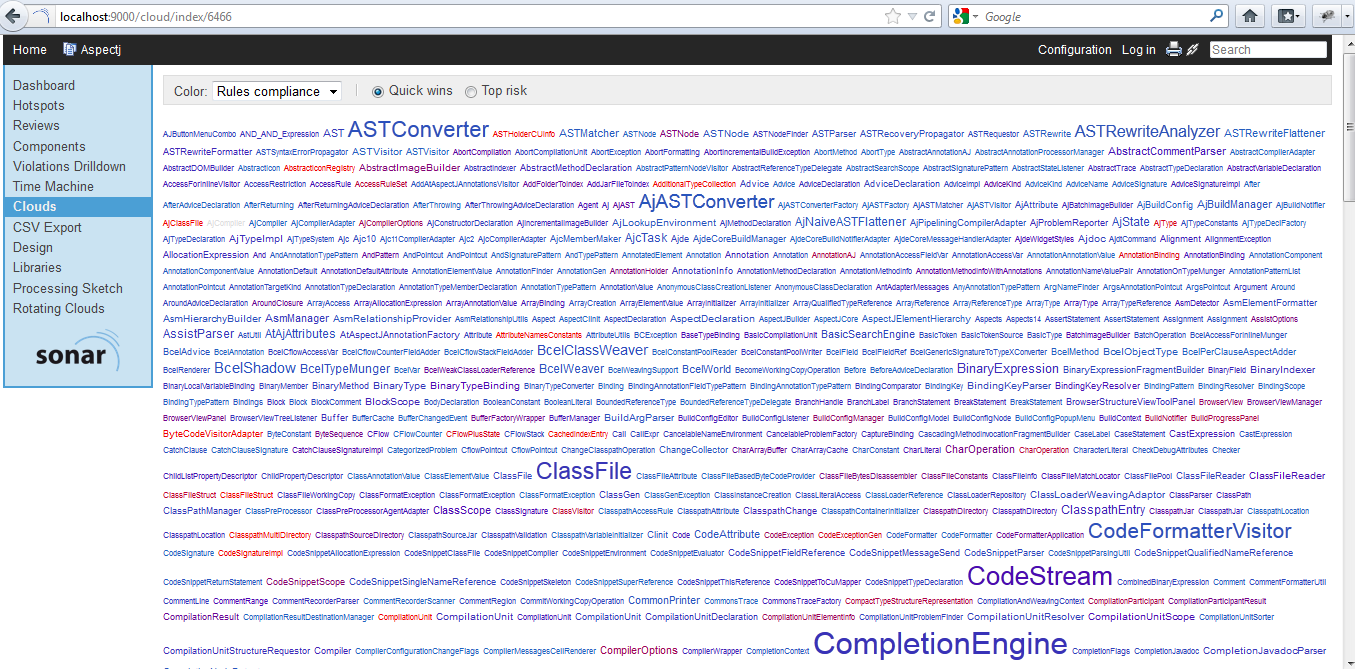
\includegraphics[width=140mm]{sonarcloud.png}
  \caption{AspectJ visualised in Sonar}
  \label{fig:aspectjsonar}
\end{figure}

\subsection{Sonar Extension using Javascript Library}

Aspectj was then visualised using a rotating 3D tag cloud component in Sonar. We created a tag cloud visualisation using Javascript library TagCanvas\footnote{\url{http://www.goat1000.com/tagcanvas.php}} and added it as a plugin into Sonar in order to use the metric data (see Fig. \ref{fig:aspectjtagcanvas}). This cloud shows the top ten most complex classes in Aspectj according to the complexity metric. With more than approximately ten class names it becomes difficult to identify the different classes. It was possible to use the tags for navigation, selecting a hyperlink to show individual metric data for the selected class named in the tag. However, navigation within a rotating 3D cloud appears particularly challenging as tags quickly rotate away from the mouse. One aspect of the visualisation which could prove useful is to prompt users of an item which requires attention. For example in a visualisation of Aspectj, the PublicScanner class name rotating to the front of the page could serve as a reminder that the class has a complexity problem that needs addressing.

\begin{figure}[h!]
   \centering
   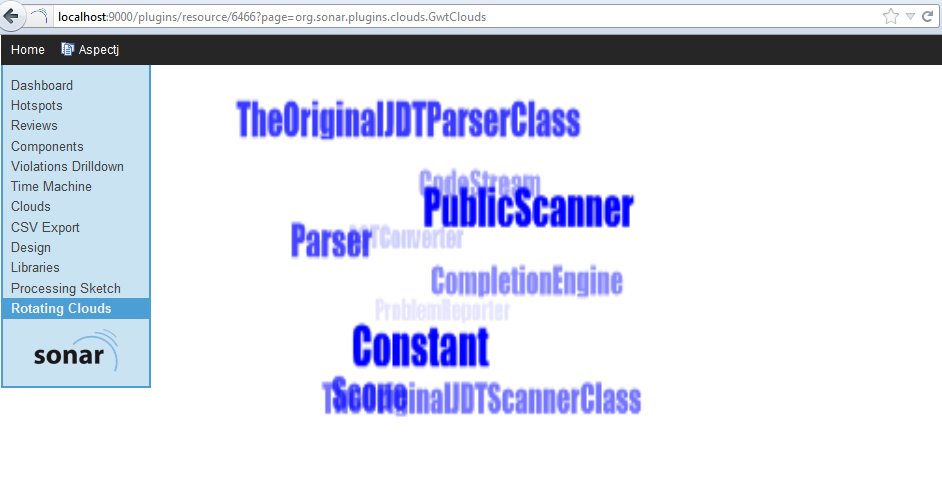
\includegraphics[width=140mm]{sonarrotatingcloud.png}
  \caption{AspectJ visualised with rotating tag cloud in Sonar}
  \label{fig:aspectjtagcanvas}
\end{figure}

%Eclipse Cloudio.
\subsection{Sourcecloud}

Eclipse plugin Sourcecloud\footnote{\url{http://misto.ch/tag/eclipse/}} produces a Wordle-like visualisation of the text within a class, package or project. Like a traditional tag cloud, words within the source are counted and font size is allocated according to the count. Colours are assigned arbitrarily. The issue of scale is approached by allowing a maximum number of words - if this is set too large for the visualisation to fit on the canvas, an error message is displayed. It is not possible to select words to exclude from the tag cloud but it is possible to highlight a specific tag. According to the Sourcecloud documentation, the tag cloud should give an impression of how easy the code base is to understand, by containing a greater proportion of domain-specific classname tags than core Java API classname tags. We produced a visualisation of the Aspectj project source code using Sourcecloud (see Fig. \ref{fig:sourcecloud}). While looking very pretty, it doesn't appear overly useful as a gauge of code quality.

\begin{figure}[h!]
   	\centering
  	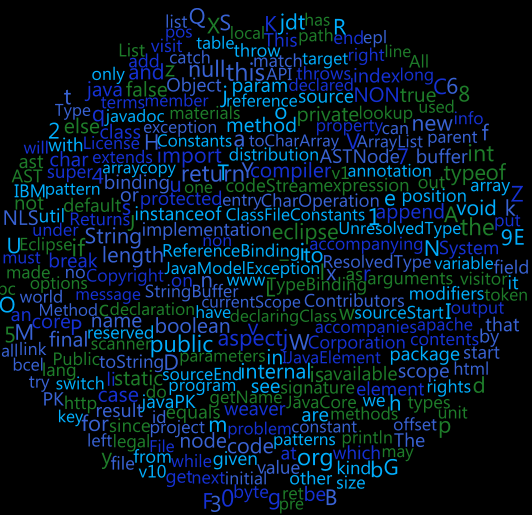
\includegraphics[width=140mm]{sourcecloud.png}	
	\caption{AspectJ source code visualised with Sourcecloud}
	\label{fig:sourcecloud}
\end{figure}

%What do they do with tag length?

%Code Gestalt

%Taggle.

\subsection{Taggle}

In order to understand whether tag clouds can enable effective visualisation of software, we must consider the following points:

\begin{itemize}
	\item Can tag clouds support the large data sets of software elements?
	\item Can the presence of outliers be easily identified within a tag cloud? %skewed data
	\item What are the limitations of tags? How can tags support long structure names or labels?
	\item What effect do cloud layout algorithms have on the user?
	\item Can tag clouds support showing software evolution over time?
	\item How effectively do tag clouds support navigation through data elements?
	\item Will the user benefit from greater interaction with a tag cloud?
	\item Can we show data element relationships with a tag cloud? %forced layout
	\item Can tag clouds be used to indicate the presence of code smells or other possible problem areas using software metrics?
	\item When is it sensible to use a tag cloud over another visualisation such as treemap or histogram?
	\item Is it useful to provide a stop list or filtering system for data elements?
	\item Is it useful to customise tags - such as alter the tag position or remove irrelevant data elements?
	\item Identification of appropriate test cases.
\end{itemize}

In previous University of Canterbury work, a prototype application `Taggle', has been built which attempts to address the specific challenges faced with visualising software in tag clouds \citep{deaker11, deaker11b, deaker11c}. This application allows mapping of multiple variables of key (user-defined) attributes. This can be built upon as a starting point to further research in this area.

\begin{figure}[h!]
   \centering
   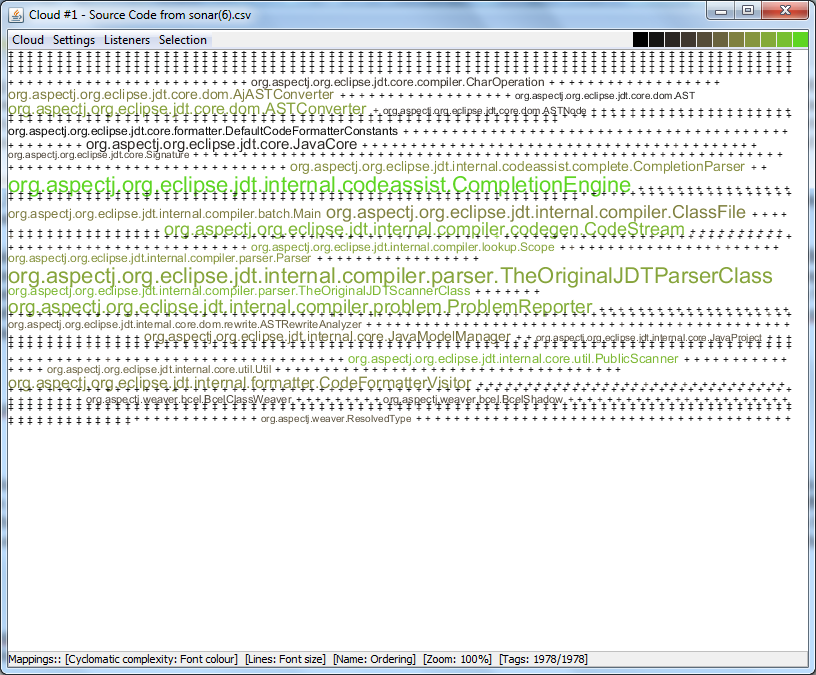
\includegraphics[width=140mm]{aspectjtaggle.png}
  \caption{AspectJ visualised in Taggle}
\end{figure}

% ------------------------------------------------------------------------

%%% Local Variables: 
%%% mode: latex
%%% TeX-master: "../thesis"
%%% End: 
